We model our ER diagram (\cref{fig:er-diagram}) after Pomona College's current
room draw system with a few modifications. Students may be members of various
draw groups, each of which must contain at least one student. 

Furthermore, each draw group must have a \emph{Representative} who
will select a \emph{Collection} of one or more rooms for the group. The collection's total
capacity must match the size of the draw group. 

Similar to the student/draw group coupling, a
\emph{Room} is required to be a part of exactly one collection. These
collections represent individual rooms by themselves and multiple associated rooms like
two-room doubles and friendship suites. A representative may \emph{Request} a
collection and rank the request for automated room draw; this set of requests and rankings makes up
the group's preference's list. The priority of a request is determined by \emph{rank\_absolute}
which is a function of a Draw Group's \emph{draw\_num} and the importance of that request for
a Draw Group relative to their other requests. 

The \emph{Occupy} relation will be set by our AutoDraw system, assigning a collection
to a Draw Group in accordance with the totally ordered set of all Requests. This allows
students in a Draw Group to later assign themselves to appropriate rooms within an 
assigned Collection in accordance with the joint decisions of the members of the Draw Group. 

\begin{figure}[H] \centering
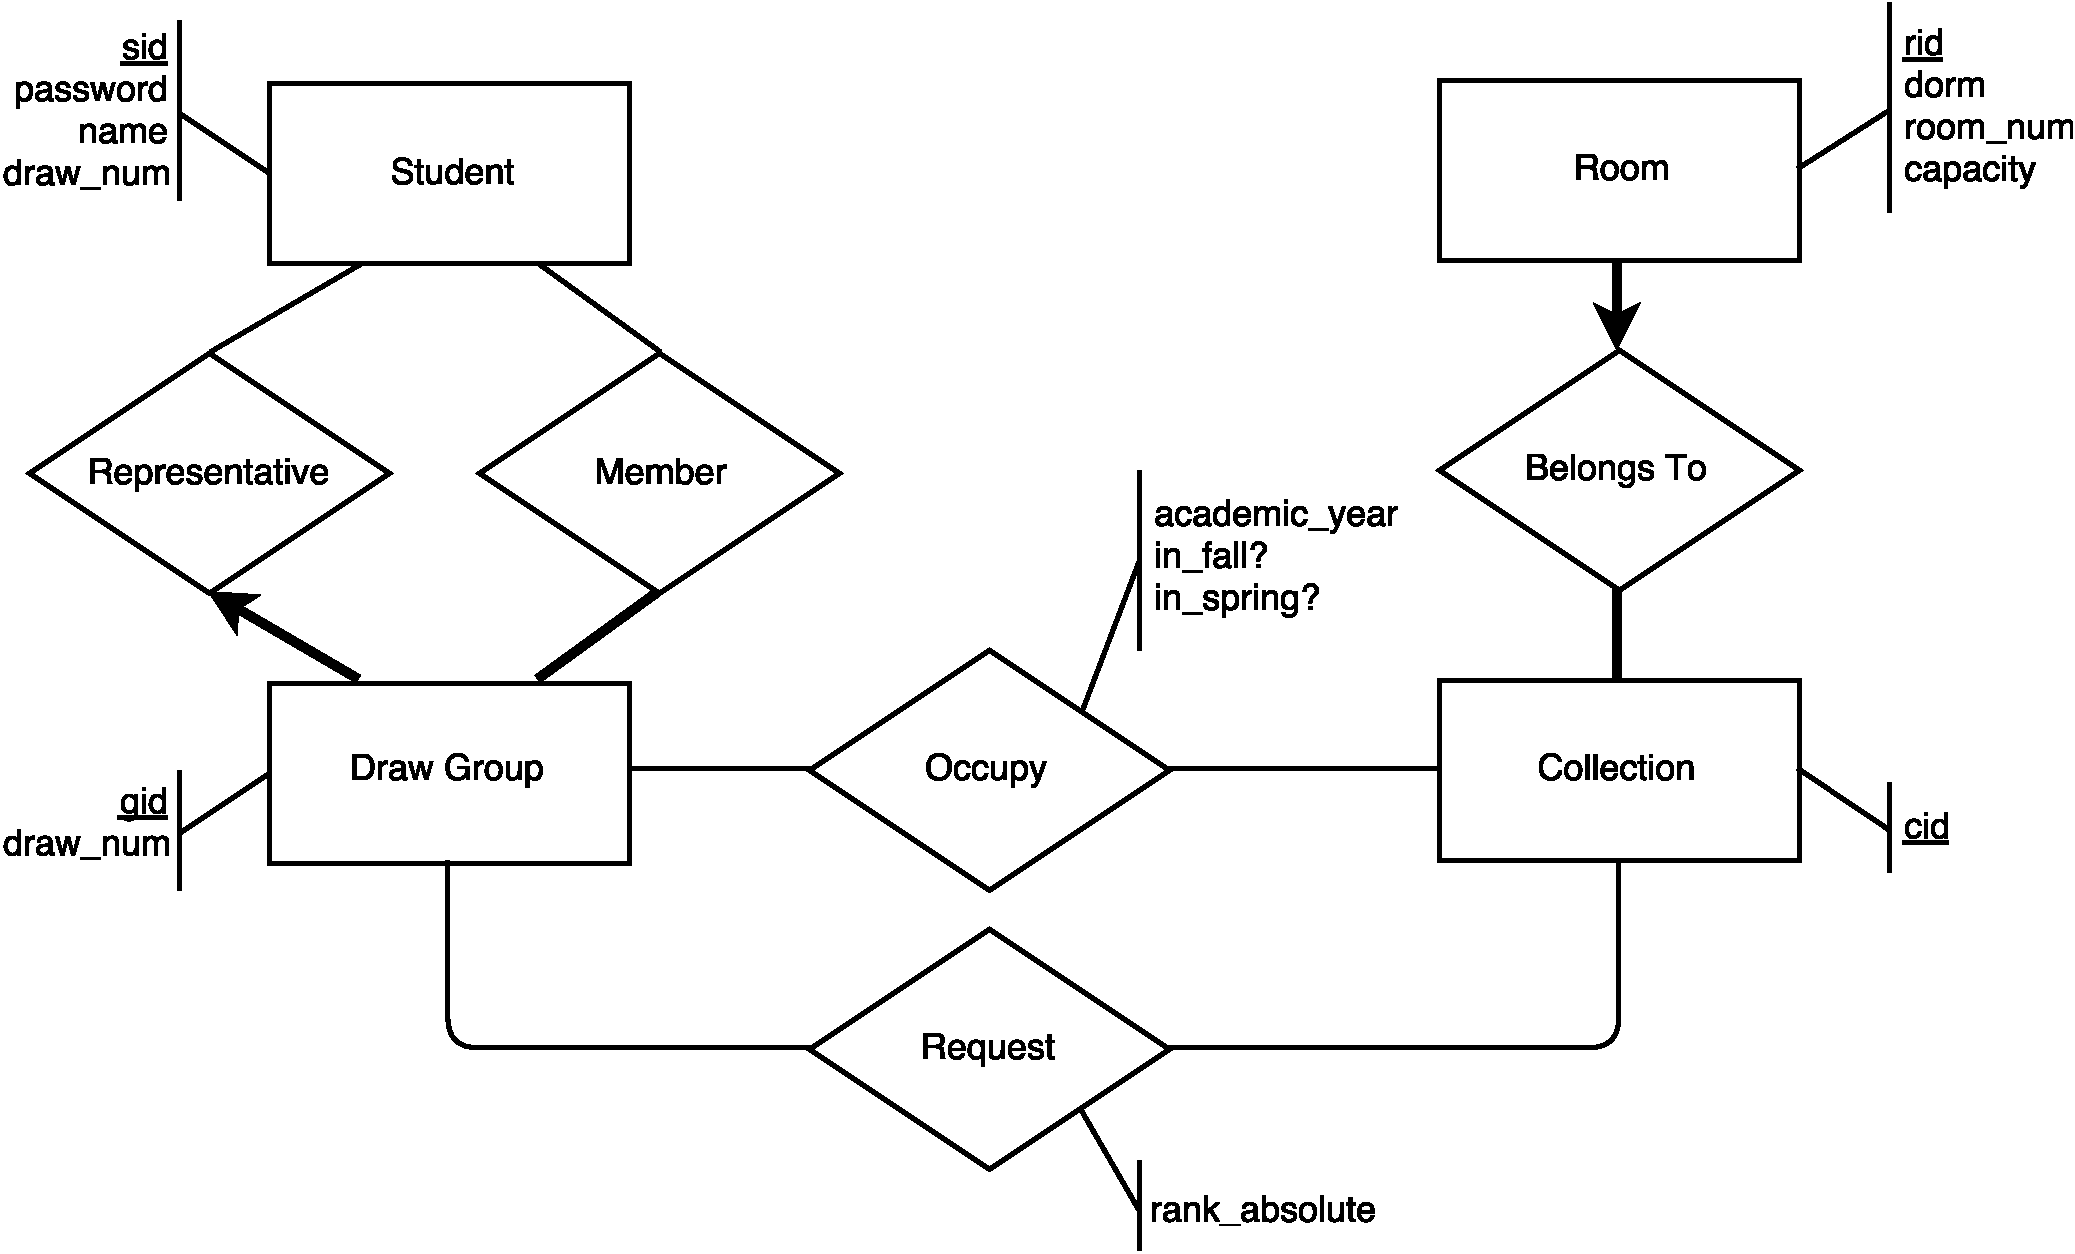
\includegraphics[width=\textwidth]{er_crop.pdf}
\caption{Our ER Diagram}
\label{fig:er-diagram}
\end{figure}
